\begin{surferPage}[Singularitat A4+-]{Una singularitat $A_4^{+-}$}
Una $A_4^{+-}$ és semblant a qualsevol singularitat de tipus
$A_{2k}^{+-}$, $k\ge 1$, com es veu mirant l'equació
    \[x^{2k+1}+y^2-z^2=0.\]
L'única diferència aparent amb una
$A_2^{+-}$ (imatge dessota a l'esquerra)
és l'ordre de tangència. Les altres dues imatges són
d'una $A_4^{+-}$ i una $A_6^{+-}$), respectivament.
    \vspace*{-0.5em}
    \begin{center}
      \begin{tabular}{c@{\quad}c@{\quad}c}
        \begin{tabular}{@{}c@{}}
          
\includegraphics[width=1.2cm]{../../common/images/A2pm}
        \end{tabular}
        &
        \begin{tabular}{@{}c@{}}
          
\includegraphics[width=1.2cm]{../../common/images/A4pm}
        \end{tabular}
        &
        \begin{tabular}{@{}c@{}}
          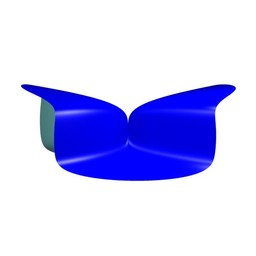
\includegraphics[width=1.2cm]{../../common/images/A6pm}
        \end{tabular}
      \end{tabular}
    \end{center}
    \vspace*{-0.4em}
Però això proporciona una diferència fonamental amb la deformació a
singularitats còniques. Ho i\l.lustrem amb
una deformació en una superfície amb forats.
Per a una $A_k^{+-}$, es poden obtenir $k$ forats, 4 en
el nostre cas (en la imatge es mostren en dos parells;
compareu amb el cas $A_2^{+-}$, ja vist abans, amb un forat).
    \begin{center}
      \vspace{-0.1cm}
      \begin{tabular}{@{}c@{\quad}c@{}}
        \begin{tabular}{@{}c@{}}
          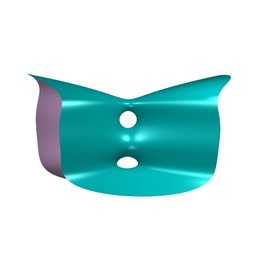
\includegraphics[width=1.2cm]{../../common/images/A4pm_sm_0}
        \end{tabular}
        &
        \begin{tabular}{@{}c@{}}
          
\includegraphics[width=1.2cm]{../../common/images/A4pm_sm_1}
        \end{tabular}
      \end{tabular}
    \end{center}
%     \dontshow{
%     %
%     \begin{center}
%       \vspace{-0.1cm}
%       \begin{tabular}{@{}c@{\quad}c@{\quad}c@{}}
%         \begin{tabular}{@{}c@{}}
%           
\includegraphics[width=1.2cm]{../../common/images/A4pm_0}
%         \end{tabular}
%         &
%         \begin{tabular}{@{}c@{}}
%           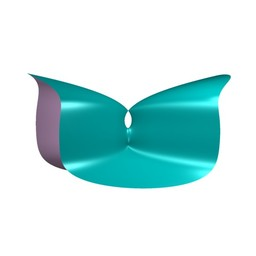
\includegraphics[width=1.2cm]{../../common/images/A4pm_1}
%         \end{tabular}
%         &
%         \begin{tabular}{@{}c@{}}
%           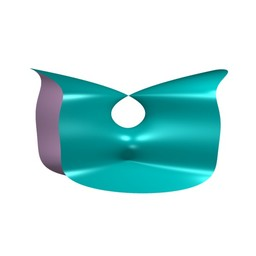
\includegraphics[width=1.2cm]{../../common/images/A4pm_2}
%         \end{tabular}
%       \end{tabular}
%     \end{center}
%     }
 
\end{surferPage}
